\chapter{Morphological diversity in tenrecs compared to golden moles}
\label{chap:disparity}


\section{Introduction}
	In Chapter \ref{chap:introduction}, I explained why it is important to study patterns of morphological diversity in tenrecs. In this chapter, I present the first quantitative investigation of morphological diversity in tenrecs. I use geometric morphometric techniques \citep{Rohlf1993} to compare cranial morphological diversity in tenrecs to that of their closest relatives, the golden moles. 
	I expect tenrecs to be more morphologically diverse than golden moles because tenrecs occupy a wider variety of ecological niches. The tenrec Family includes terrestrial, semi-fossorial, semi-aquatic and semi-arboreal species \citep{Soarimalala2011}. In contrast, all golden moles occupy very similar, fossorial ecological niches \citep{Bronner1995}. 
	Greater ecological variety is often (though not always) correlated with higher morphological diversity \citep{Losos2010a}. In this chapter I test whether this prediction is supported when I compare morphological diversity in tenrecs to golden moles.

%------------------------------------------------------
\section{Methods}

	The methods I used to measure morphological diversity involved several steps of data collection, processing and analysis. For clarity,  Figure \ref{fig:flow} summarises all of these steps and I describe them in detail below. Note that I repeated the same analyses for each of the different sets of photographs: skulls in dorsal, ventral and lateral views, and mandibles in lateral view.
	
%*************************************************
%Methods flowchart: 
%**************************************
	%SF: I've changed parts of this compared to the chart in the paper manuscript but the overall steps are the same because I'm hoping that the new description in the text makes them clearer.
		\begin{figure}[!htbp]
		\centering
		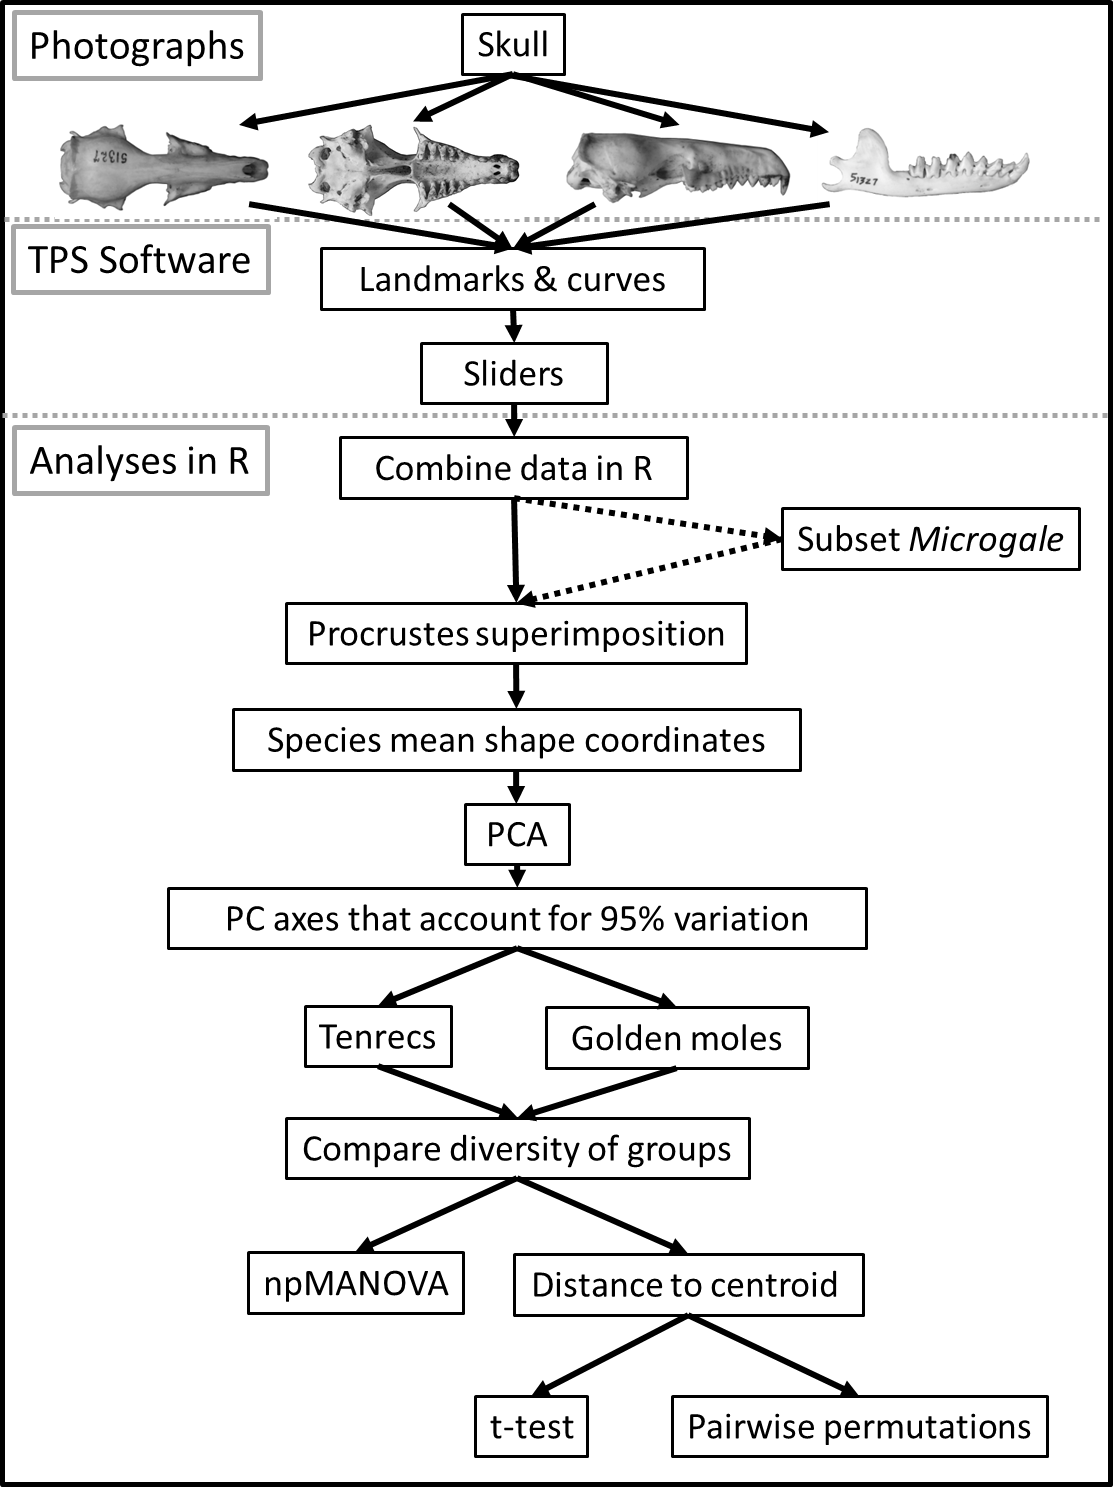
\includegraphics[width=1\linewidth,height=0.8\textheight]{Disparity/writing/figures/Methods_flowchart_thesis.png}
		
		\caption[Flowchart diagram of data collection and analysis]
			{Summary of the main steps in my data collection, processing and analysis protocol. Note that the analyses were repeated separately for each set of photographs: skulls in dorsal, ventral and lateral views and mandibles in lateral view. The dashed arrows refer to the stage at which I selected a subsample of the tenrecs (including just five species of the \textit{Microgale} Genus) so that I could compare the morphological diversity of this reduced subsample of tenrec species to the diversity of golden moles.}
		
		\label{fig:flow}
		\end{figure}
%----------------------------------------------------	

	In Chapter \ref{chap:methods} (Figure \ref{fig:flow}), I described how I photographed skulls and summarised their morphologies using landmark morphometrics. I used photographs of 182 skulls in dorsal view (148 tenrecs and 34 golden moles), 173 skulls in ventral view (141 tenrecs and 32 golden moles), 171 skulls in lateral view (140 tenrecs and 31 golden moles) and 181 mandibles in lateral view (147 tenrecs and 34 golden moles). These samples represent 31 species of tenrec (out of the total 34 in the Family; \citealp{Olson2013}) and 12 species of golden moles (out of a total of 21 species in the Family; \citealp{Asher2010}). Note that the number of skulls I used varies slightly for each analysis because some skulls were damaged in certain views.
	

	After placing the landmarks and creating sliders files within the TPS software series (Chapter \ref{sect:morphometrics}, Figure \ref{fig:flow}), I combined the files into a single morphometrics data object and carried out all further analyses in R version 3.1.1 \citep{Team2014} and my code is available on GitHub \citep{Finlay2015c}. At this stage, I either used the full data set (31 species of tenrec and 12 species of golden mole) or a reduced data set with just 17 species of tenrec. I created this reduced data set because the majority of tenrec species (19 out of 31 in my data) belong to the \textit{Microgale} (shrew-like) Genus that has relatively low morphological diversity \citep{Soarimalala2011, Jenkins2003}. This may mask signals of higher morphological diversity among other tenrecs. To test this, I created a subset of the tenrec data that included just five of the \textit{Microgale} species, each representing one of the five sub-divisions of \textit{Microgale} outlined by Soarimalala and Goodman \citeyearpar{Soarimalala2011}, i.e. small, small-medium, medium, large and long-tailed species. I compared the morphological diversity of this subset of tenrecs (n=17: five \textit{Microgale} and 12 non-\textit{Microgale} species) to that of the 12 species of golden moles (dashed arrows in Figure \ref{fig:flow}). After this selection stage, all further steps in the analyses were the same.
		
	For each analysis, I did a general Procrustes alignment of the shape data and calculated the mean shape coordinates for every species (see section \ref{sect:procrustes}). I used these average, Procrustes-superimposed shape coordinates for a principal components analysis (PCA) and then selected the number of principal component (PC) axes that accounted for 95\% of the variation in the data (Figure \ref{fig:flow}). Selecting the number of PC axes based on their cumulative variance \citep[e.g.][]{Brusatte2008, Collar2006} rather than through an arbitrary cut off standardised my diversity comparisons across the different analyses.
	
\subsection{\normalfont{Estimating morphological diversity}}
	
	I grouped the PC scores for tenrecs and golden moles separately so that I could estimate the diversity of each Family and then compare the two groups (Figure \ref{fig:flow}). I compared morphological diversity in two ways. First, I used non parametric multivariate analysis of variance \citep[npMANOVA;][]{Anderson2001} to test whether tenrecs and golden moles occupied significantly different positions within the morphospaces defined by the PC axes that accounted for 95\% of the overall variation in the data \citep[e.g.][]{Serb2011, Ruta2013}. A significant difference between the two Families would indicate that they have unique morphologies which do not overlap. Second, I compared morphological diversity within tenrecs to the diversity within golden moles. I define morphological diversity as the mean Euclidean distance (sum of squared differences) between each species and its Family centroid (Figure \ref{fig:centroids}). This is summarised in the equation below where \textit{n} is the number of species in the Family, \textit{i} is the number of PC axes and \textit{c} are the average PC scores for each axis (the centroid). 
	
	\begin{equation}
	Diversity = \frac{\sqrt{\Sigma(PCn_{i}-PCc_{i})^2}}{n}
	\end{equation}

	
	
	If tenrecs are more morphologically diverse than golden moles, then they should be more dispersed within the morphospaces and have, on average, higher values of mean Euclidean distance. 
	

%-----------------------------
%Diagram of mean distance to centroid (based on the diagram in Cooper et al 2009)
	\begin{figure}[!htbp]
	\centering
	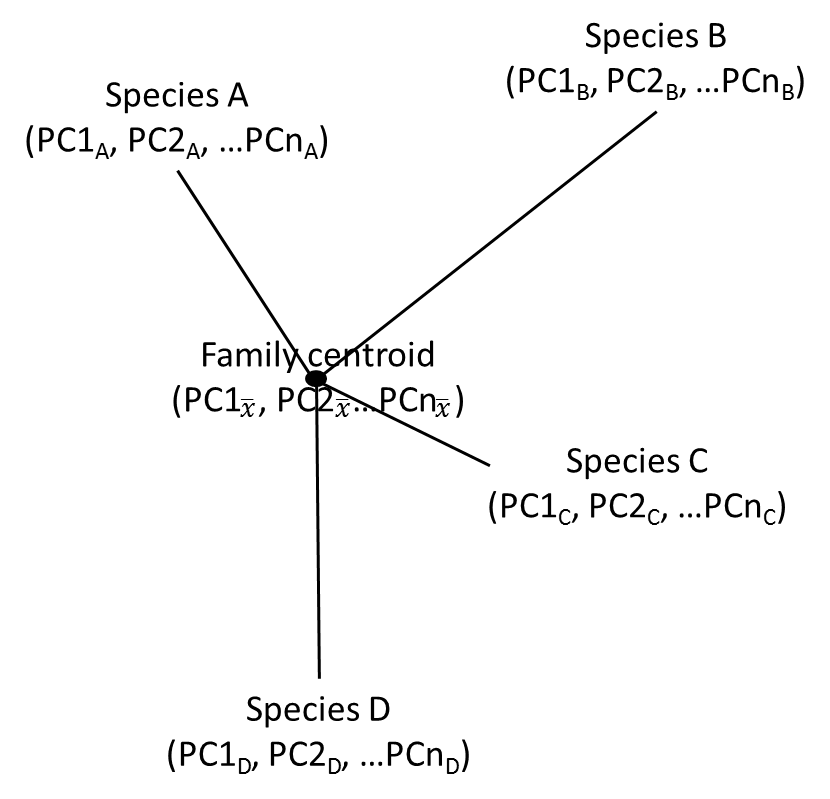
\includegraphics [width=0.7\linewidth, height=0.7\textheight, keepaspectratio]{Disparity/writing/figures/Centroids.png}
	\caption[Calculating diversity as mean Euclidean distance to Family centroid.]
		{Estimating morphological diversity as the mean Euclidean distance between each species and the Family centroid. Every species had scores on the principal components (PC) axes that accounted for 95\% of the variation in the principal components analysis. The number of axes (PCn) varied for each analysis but they were the same within a single analysis. PC scores were used to calculate the Euclidean distance from each species to the Family centroid (average (\begin{math}
			\bar{x}
			\end{math}) PC scores for the entire Family). Morphological diversity of the Family is the average value of these Euclidean distances.}
	\label{fig:centroids}
	\end{figure}
% SF: I moved the text and made the lines into double headed arrows, the error bar-type endings looked messy	

%--------------------------------------

	
	One possible issue with these analyses is that the two Families have unequal sample sizes: 31 (or a subset of 17) tenrec species compared to just 12 golden mole species. Morphological diversity is usually decoupled from taxonomic diversity \citep[e.g.][]{Ruta2013, Hopkins2013} so larger groups are not necessarily more morphologically diverse. However, comparing morphological diversity in tenrecs to the diversity of a smaller Family could still bias the results: overall diversity in tenrecs could be higher if diversity is simply a function of sample size. As described in the paragraph below, I used pairwise permutation tests to account for this potential issue. 

	I tested the null hypothesis that tenrecs and golden moles have the same morphological diversity (the same mean Euclidean distance to the Family centroid). If this is true, when you randomly assign the group identity of each species (i.e. shuffle the "tenrec" and "golden mole" labels) and then re-compare the morphological diversity of the two groups, there will be no significant difference between these results and those obtained when the species are assigned to the correct groupings. 
	% NC: I've rephrased this as really what is happening here is that there is no difference between the results you get with proper groupings versus random groupings. You expect that random groupings give no difference.
	I performed this shuffling procedure (random assignation of group identity) 1000 times and calculated the difference in morphological diversity between the two groups for each permutation. This generated a distribution of 1000 values which are calculations of the differences in morphological diversity under the assumption that the null hypothesis (equal morphological diversity in the two Families) is true. This method automatically accounts for differences in sample size because shuffling of the group labels preserves the sample size of each group: there will always be 12 species labelled as "golden mole" and then, depending on the analysis, either 31 or 17 species labelled as "tenrec". Therefore, the 1000 permuted values of differences in morphological diversity create a distribution of the expected difference in diversity between a group of sample size 31 (or 17 in the case of the subsetted tenrec data) compared to a group of sample size 12 under the null hypothesis that the two groups have the same morphological diversity. I compared the observed measures of the differences in morphological diversity between the two Families to these null distributions to determine whether there were significant differences after taking sample size into account (two-tailed t test).
	
%----------------------------------------------------

\section{Results}
\label{sect:results}

	Figure \ref{fig:FourPCA} depicts the morphospaces defined by the first two principal component (PC) axes from my principal components analyses (PCAs) of skull and mandible morphologies. The PCAs are based on the average Procrustes -\\superimposed shape coordinates for skulls in three views (dorsal, ventral and lateral) and mandibles in lateral view.

%-----------------------------
% SF: I took away the silhouette legend
	
%PCA figure
	%From the twofamily_disparity_PCAplots script
	\begin{figure}[!htbp]
	\centering
	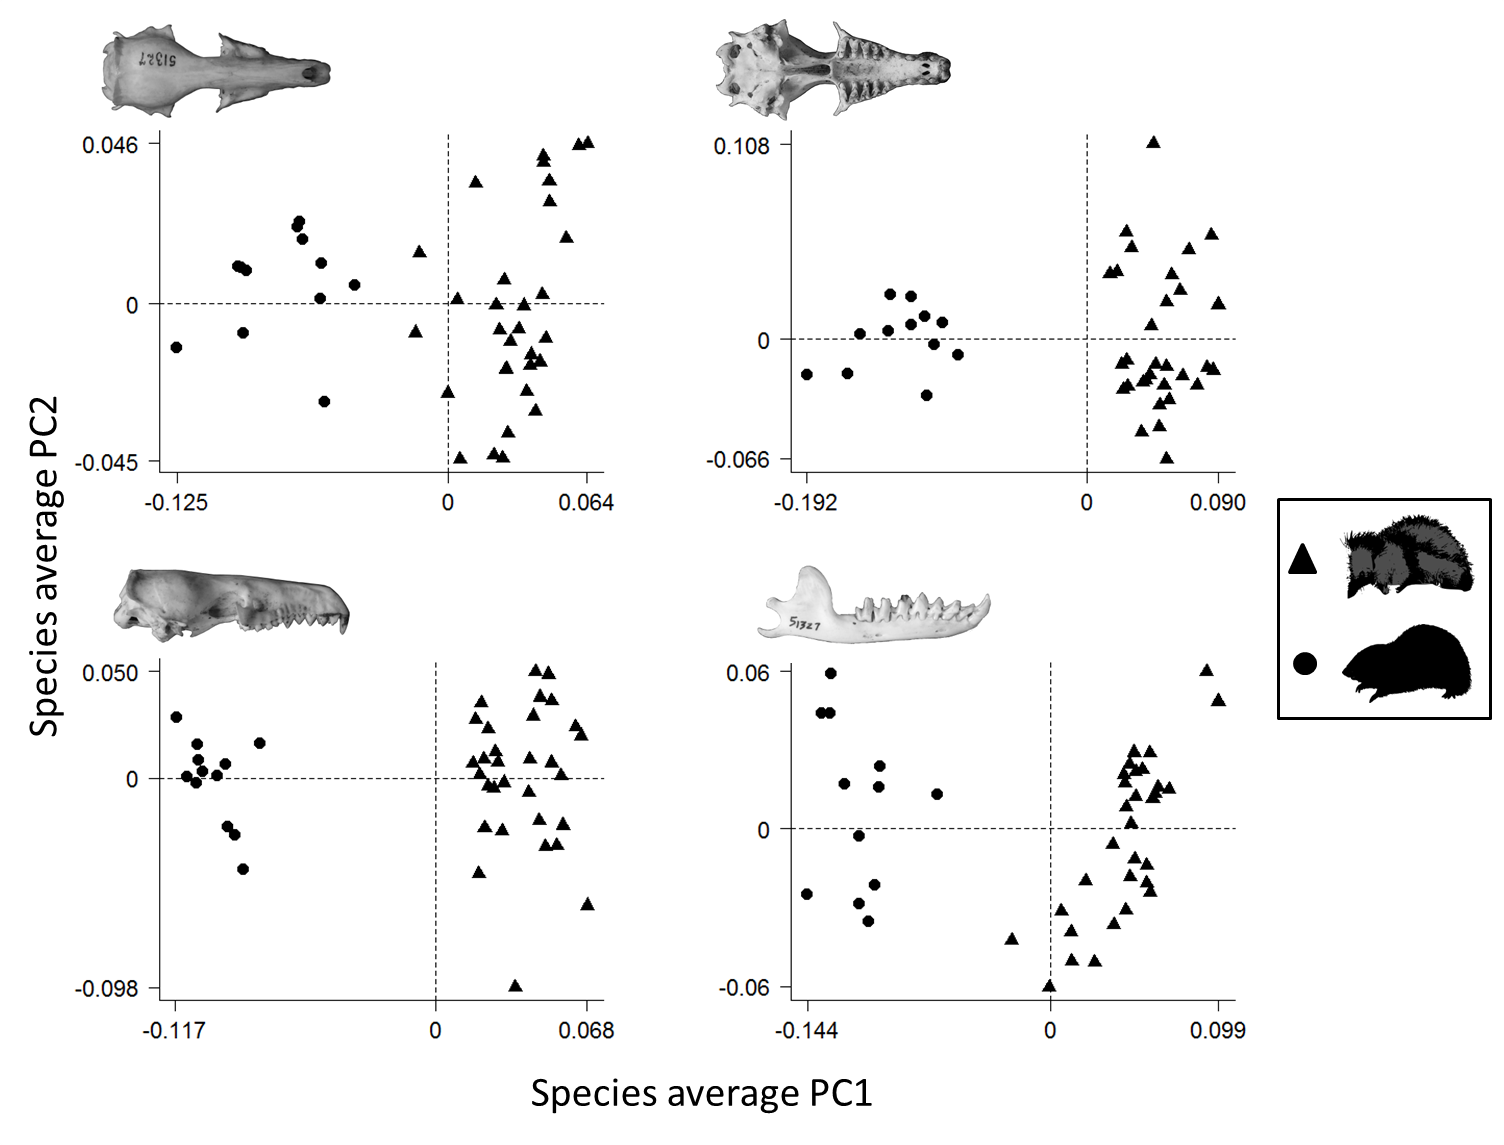
\includegraphics[width=1\linewidth, height=1\textheight, keepaspectratio]{Disparity/writing/figures/FourPCA_shapes.png}
	\caption[Morphospace (principal components) plot of morphological diversity in tenrec and golden mole skulls.]
		{Principal components plots of the morphospaces occupied by tenrecs (triangles, n=31 species) and golden moles (circles, n=12 species) for the skulls in dorsal (top left), ventral (top right) and lateral (bottom left) views, and mandibles in lateral view (bottom right). Each point represents the average skull shape of an individual species. Axes are principal component 1 (PC1) and principal component 2 (PC2) of the average scores from principal components analyses of mean Procrustes shape coordinates for each species.}
	\label{fig:FourPCA}
	\end{figure}
%----------------------------------------------

	To compare morphological diversity in the two families, I used the PC axes which accounted for 95\% of the cumulative variation in each of the skull analyses: dorsal (n=6 axes), ventral (n=7 axes) and lateral (n=7 axes) and the mandibles (n=11 axes). First, I compared the position of each Family within the morphospace plots. Tenrecs and golden moles occupy significantly different positions in the dorsal (npMANOVA: F\textsubscript{1,42}=68.13, R$^2$=0.62, p=0.001 ), ventral (npMANOVA: F\textsubscript{1,42}=103.33, R$^2$=0.72 , p=0.001 ) and lateral (npMANOVA: F\textsubscript{1,42}=76.7, R$^2$ =0.65, p=0.001 ) skull morphospaces as well as in the mandible morphospace (npMANOVA: F\textsubscript{1,42}=60.38, R$^2$=0.59, p=0.001),  indicating that the Families have very different, non-overlapping cranial and mandible morphologies (Figure \ref{fig:FourPCA}). 

	
	%SF: I changed the text to have no spacing around = and the tables have spaces around the +/- because otherwise it looks too cluttered
	
	%Numbers are from the npMANOVA based on PC axes within my diversity_twofamily_cent_dist script
%----------------------------------------
%Results table: I changed the format to make it fit better
\begin{landscape}
	\begin{table}[!htbp]			
		\caption[Comparing morphological diversity in tenrecs and golden moles.]
		{Morphological diversity in tenrecs compared to golden moles (12 species). N is the number of tenrec species: 31 species or 17 species including just five representatives of the \textit{Microgale} Genus. Morphological diversity of the Family is the mean Euclidean distance from each species to the Family centroid. Significant differences between the two Families (p$<$0.05) from two-tailed t-tests are highlighted in bold.}
		%Diversity based on centroid distances results summary
%All tenrecs and golden moles
%Morphological diversity based on comparing the mean Euclidean distances to each family's centroid
%NB: degrees of freedom are different in each analysis because I'm using a Welch two sample t test: df comes from a distribution of values based on the error within each sample so the final numbers will be different for each data set

%Re-ordered the table so that everything would fit in better


\resizebox{\columnwidth}{!}{
%Scales down the table to fit within the column width
	% If this is too small then I'll probably need to break the table into two
\begin{tabular}{c l c c c c}		
\hline
N& Analysis & \multicolumn{2}{c}{Morphological diversity} & t\textsubscript{df} & p value\\
%-----------------------------------------------
\hline
%------------------------
 &  & Tenrecs  & Golden moles &  &  \\
%--------------------------------
\cline{3-4} % Puts a line just through some columns
%---------------------------------
 & & (mean $\pm$ s.e) & (mean $\pm$ s.e) & &\\
\hline
%\multicolumn{1}{l}
%---------------------------
 31 & Skulls dorsal & \multicolumn{1}{l}{0.036 $\pm$ 0.0029} & 0.029 $\pm$ 0.0032 & -1.63\textsubscript{29.88}& 0.11 \\
%--------------------------------------
 & Skulls ventral & \multicolumn{1}{l}{0.048 $\pm$ 0.0034} & 0.044 $\pm$ 0.0041 & -0.68\textsubscript{26.99} & 0.51\\
%-----------------------------------------
 & Skulls lateral & 0.044 $\pm$ 0.0041 & 0.032 $\pm$ 0.0037 & -2.16\textsubscript{35.03} & \textbf{0.04}\\
%----------------------------------------
 & Mandibles & 0.049 $\pm$ 0.0044 & 0.067 $\pm$ 0.0054 & 2.62\textsubscript{25.85} & \textbf{0.01}\\
%--------------------------
\hline
%-----------------------------------------
17 & Skulls dorsal & 0.044 $\pm$ 0.0025 & \multicolumn{1}{l}{0.029 $\pm$ 0.0032} & -3.62\textsubscript{22.75} & \textbf{<0.01}\\
%---------------------------------
 & Skulls ventral & \multicolumn{1}{l}{0.054 $\pm$ 0.0039} & \multicolumn{1}{l}{0.042 $\pm$ 0.0041} & -2.23\textsubscript{25.46} & \textbf{0.04}\\
%-------------------------------------
 & Skulls lateral &  \multicolumn{1}{l}{0.054 $\pm$ 0.0053} & 0.031 $\pm$ 0.0037 & -3.47\textsubscript{26.31} & \textbf{<0.01} \\
%--------------------
 & Mandibles & 0.055 $\pm$ 0.0049 & \multicolumn{1}{l}{0.062 $\pm$ 0.0050} & 1.00\textsubscript{25.88} & 0.33 \\
%--------------------

\hline
\end{tabular}
} 
		\label{tab:diversity}  
	\end{table}
\end{landscape}

%SF I fixed the number of figures, removed brackets for df and added the extra column heading
%------------------------------------

	Secondly, I compared the morphological diversity within each Family. Based on my measures of mean Euclidean distance to the Family centroids, tenrec skulls are more morphologically diverse than golden mole skulls when they are measured in lateral view but not in dorsal or ventral view (Table \ref{tab:diversity}). In contrast, when I analysed morphological diversity of skulls within the sub-sample of 17 tenrecs (including just five \textit{Microgale} species) compared to the 12 golden mole species, I found that tenrec skulls were significantly more morphologically diverse than golden moles in all analyses (Table \ref{tab:diversity}).
		
	The results of my analyses of the mandibles were different to those for the skulls. In the full analysis (31 species of tenrec compared to 12 species of golden mole), I found that golden moles have significantly more diverse mandible shapes than tenrecs but this difference was not significant when I used just 17 tenrec species (Table \ref{tab:diversity}). I recognised that my landmarks and curves for the mandibles focus particular attention on the ascending ramus (condyloid, condylar and angular processes, Figure \ref{fig:sklat_mands}). Therefore, I  deleted the three semilandmark curves around these structures and repeated my comparison of morphological diversity in the two Families. In this case, I found no significant differences in morphological diversity between the two Families (t-test, t\textsubscript{26.099}=1.709, p=0.099). Therefore, my results seem to indicate that golden moles have greater morphological variation in the posterior structures of their mandibles compared to tenrecs.
	
	The pairwise permutation tests for each analysis confirmed that differences in morphological diversity were not artefacts of differences in sample size (Table \ref{tab:permutations}). I discuss my results further in Chapter \ref{chap:discussion}.

%------------------------------------------------------
%Added the permutation results
% NC: I've shortened this a bit
\begin{landscape}
\begin{table}[!htbp]			
	\caption[Results of the permutation tests]{Results of the permutation analyses comparing the observed differences in morphological diversity to a null distribution of expected results. Morphological diversity of the Family is the mean Euclidean distance from each species to the Family centroid. Results are shown for both the full (N=31 species of tenrec compared to 12 species of golden mole) and reduced (N=17 species of tenrec compared to 12 golden moles) data sets. Significant values (p$<$0.05) indicate that the observed morphological diversity is different to the expected differences under a null hypothesis of equivalent diversities in the two Families.}
	%Combined table of permutation results

\resizebox{\columnwidth}{!}{
\begin{tabular}[t]{l l c c c c c c c}		
\hline
%------------------------------------------
N & Analysis & \multicolumn{5}{c}{Morphological diversity} & p value\\
%-------------------
\hline
%-------------------------------------------
 &  & \multicolumn{3}{c}{Measured values}& \multicolumn{2}{c}{Permuted values} &  \\
%---------------
\cline{3-7}
%-----------------
& & Tenrecs & Golden moles & Difference & Min. & Max. & \\
\hline
%--------------------------------------------------------
31 & Dorsal & 0.036 & 0.029 & 0.007 & -0.011 & 0.0098 &  0.013 \\
%--------------------------------------------------------
& Ventral &  0.048 & 0.044 & 0.0036 & -0.014 & 0.013 &  0.023\\
%--------------------------------------------------------
& Lateral & 0.044 & 0.032 & 0.012 & -0.012 & 0.011 & <0.001 \\
%--------------------------------------------------------
& Mandibles & 0.049 & 0.067 & 0.018 & -0.008 & 0.009  & <0.001 \\
%-----------------------------
\hline
%--------------------------------------------------------
17 & Dorsal & 0.044 & 0.029 & 0.015 & -0.011 & 0.014 &  <0.001 \\
%--------------------------------------------------------
& Ventral &  0.054 & 0.042 & 0.013 & -0.017 & 0.019 &  0.023 \\
%--------------------------------------------------------
& Lateral & 0.054 & 0.0313 & 0.022 & -0.018 & 0.0186 & <0.001 \\
%--------------------------------------------------------
& Mandibles & 0.055 & 0.0623 & 0.007 & -0.012 & 0.011 & 0.038\\
%-----------------------------
\hline
\end{tabular}
} 
	\label{tab:permutations}  
\end{table}
\end{landscape}


%SF: I got rid of the bold and added the extra column heading, I still need to fix the positioning
%----------------------------------------------------
% NC: The positioning of the tables is a bit weird. Perhaps play around with the float options once this is all ready so that you can try and get this looking a bit neater.
	





